\begin{frame}[fragile]{Research Questions}
    \begin{itemize}
      \setlength\itemsep{2em}
        \item Does \acrshort{dpbt} generate \textbf{incremental results} regardless of the size of the graph?
        \item Does the type of query \textbf{$Q$ impact} on the execution of \acrshort{dpbt}?
        \item How effectively \acrshort{dpbt} implements a \textbf{\emph{pay-as-you-go} model}?
        \item Does \acrshort{dpbt} handle \textbf{memory and threads} efficiently?
    \end{itemize}        
\end{frame}

\begin{frame}[fragile]{Experiments}
    \begin{itemize}
      \setlength\itemsep{2em}
      \item \textbf{Continuous behavior Analysis}: using \acrshort{dt} and \acrshort{dk} to assess the continuous behavior capabilities.
      \item \textbf{Benchmark Analysis}: to identify how the behavior of \acrshort{dpbt} varies depending on the type of query command.
      \item \textbf{Performance Analysis} \acrfull{ghc} Profiling for one of the graphs to measure multithreading and memory allocation. 
    \end{itemize}
\end{frame}

\begin{frame}[fragile]{Experiment Configuration}
  \begin{block}{Datasets Tested}
    \begin{table}[H]
      \centering
      \resizebox{1\textwidth}{!}{
      \begin{tabular}{|p{0.25\linewidth}|c|c|c|c|c|}
        \hline
       \textbf{Network} & \textbf{$|U|$} & \textbf{$|L|$} & \textbf{$|E|$} & \textbf{Wedges} & \textbf{\#\acrshort{bt}} \\
       \hline
       \rowcolor{yellow!35}
       Dbpedia & 18422 & 168338 & 233286 & $1.45 \times 10^8$ & \color{red}\bf$3.62 \times 10^8$\\
       \hline
       Moreno Crime & 829 & 551 & 1476 & 4816 & 211\\
       \hline
       \rowcolor{yellow!35}
       Opsahl UC Forum  & 899 & 522 & 33720 & 174069 & \color{red}\bf$2.2 \times 10^7$ \\
       \hline
       Wang Amazon & 26112 & 799 & 29062 & $3.4 \times 10^6$ & 110269\\
       \hline
      \end{tabular}
      }
     \end{table}
  \end{block}
  \begin{block}{Hardware Environment}
    \begin{itemize}
          \item \emph{HPC Cluster at UPC}
          \item $x86$ $64$ bits
          \item $24$-Core Intel(R) Xeon(R) CPU X5650 processor of $2.67$ GHz
          \item \emph{Hyper-threading} enable
          \item $40 GB$ up to $120 GB$ of RAM for the biggest \acrfull{dbpedia} graph
      \end{itemize}        
  \end{block}
\end{frame}

\begin{frame}[fragile]{Experiment Configuration}
  \begin{block}{Test Case Scenarios}
    \begin{table}[H]
      \centering
      \resizebox{1\textwidth}{!}{
        \begin{tabular}{|l|c|c|}
          \hline
          \textbf{Scenario ID} & \textbf{Name} & \textbf{Search by}\\
          \hline
          E-H & Edge High & edge with high incidence \\
          \hline
          E-L & Edge Low & edge with low incidence \\
          \hline
          E-M & Edge Medium & edge with medium incidence \\
          \hline
          VL-H & $l \in L$ High & vertex in lower layer with high incidence \\
          \hline
          VL-L & $l \in L$ Low & vertex in lower layer with low incidence \\
          \hline
          VL-M & $l \in L$ Medium & vertex in lower layer with medium incidence \\
          \hline
          VU-H & $u \in U$ High & vertex in upper layer with high incidence \\
          \hline
          VU-L & $u \in U$ Low & vertex in upper layer with low incidence \\
          \hline
          VU-M & $u \in U$ Medium & vertex in upper layer with medium incidence \\
          \hline
        \end{tabular}
    }
     \end{table}
  \end{block}
\end{frame}

\begin{frame}[fragile]{E1: Continuous Behavior: \acrshort{dt} and \acrshort{dk}}
  \begin{table}[H]
    \centering
    \resizebox{1\textwidth}{!}{
    \begin{tabular}{|p{0.25\linewidth}|c|c|c|}
      \hline
     \textbf{Network} & \textbf{Scenario ID} & \textbf{\acrshort{dt} Metric}  & \textbf{\acrshort{dk} Metric}\\
     \hline
     \multirow{3}{*}{Moreno Crime}
      & VU-H & $6.05 \times 10^2$ & $0.00$\\
      & VL-H & $7.95 \times 10^3$ & $0.00$\\
      & E-H & $9.85 \times 10^3$ & $0.00$\\
      \hline
      \multirow{3}{*}{Dbpedia}
      & VU-H & $3.32 \times 10^{13}$ & $1.97 \times 10^5$\\
      & VL-H &  $1.81 \times 10^{14}$ & $2.34 \times 10^4$\\
      & E-H &  $1.75 \times 10^{13}$ & $3.28 \times 10^5$\\
      \hline
      \multirow{3}{*}{Opsahl UC Forum}
      & VU-H &  $1.99 \times 10^{12}$ & $1.27 \times 10^5$\\
      & VL-H &  $6.44 \times 10^{11}$ & $1.90 \times 10^5$\\
      & E-H &  $1.02 \times 10^{11}$ & $2.93 \times 10^5$\\
      \hline
      \multirow{3}{*}{Wang Amazon}
      & VU-H & $1.50 \times 10^7$ & $43.6$\\
      & VL-H & $2.24 \times 10^7$ & $63.1$\\
      & E-H & $8.06 \times 10^6$  & $42.3$\\
      \hline
    \end{tabular}
    }
   \end{table}
\end{frame}

\begin{frame}[fragile]{E1: Continuous Behavior: \acrshort{dt} and \acrshort{dk}}
  \begin{figure}[!htp]
    \centering
    \begin{subfigure}[t]{0.45\textwidth}
     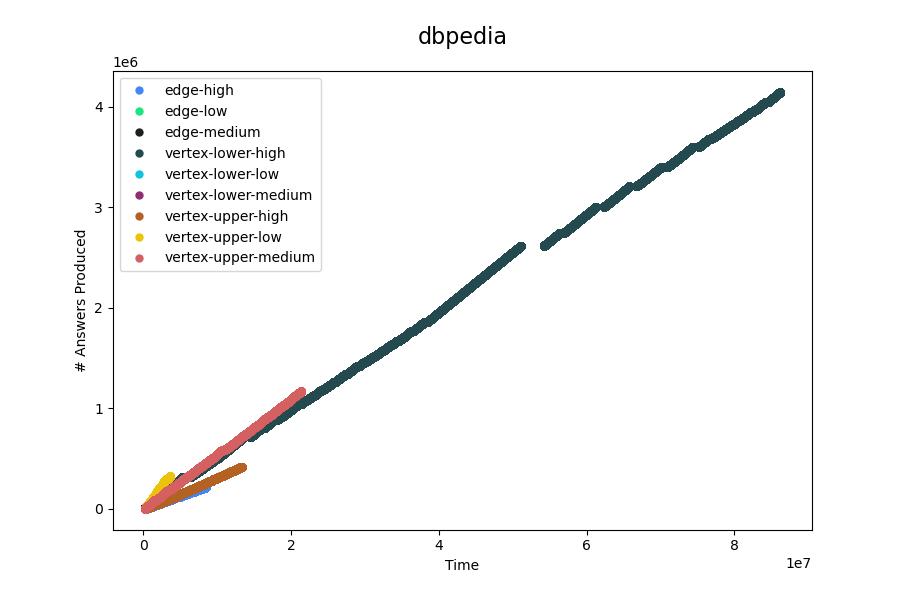
\includegraphics[width=1\linewidth, height=0.4\textheight]{experiments/diepfy/dbpedia.png}
    \end{subfigure}\hfill
    \begin{subfigure}[t]{0.45\textwidth}
     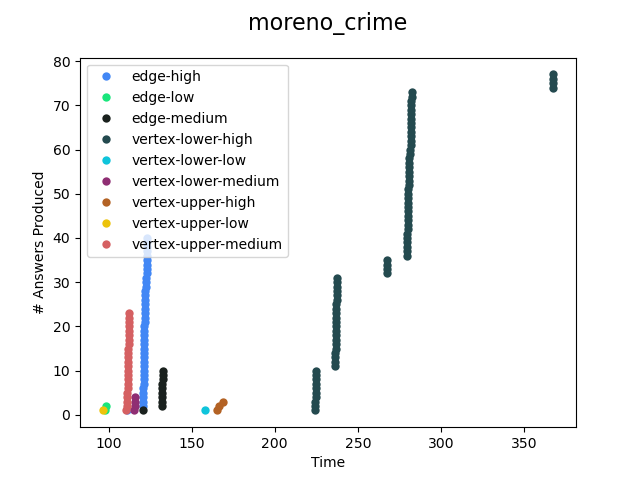
\includegraphics[width=1\linewidth, height=0.4\textheight]{experiments/diepfy/moreno_crime.png}
    \end{subfigure}
    \vspace{0.5cm}
  
    \begin{subfigure}[t]{0.45\textwidth}
     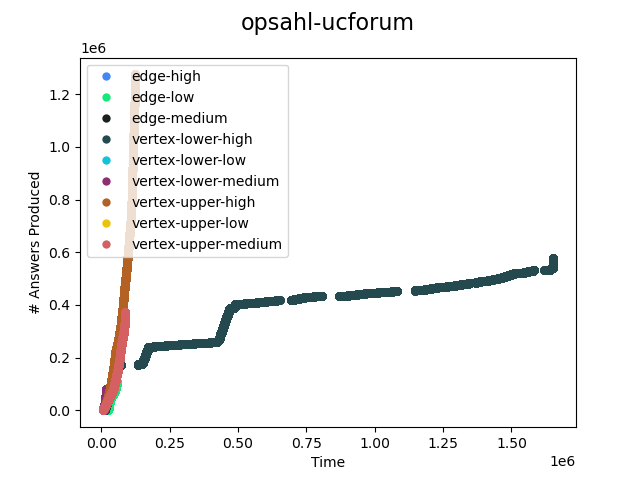
\includegraphics[width=1\linewidth, height=0.4\textheight]{experiments/diepfy/opsahl-ucforum.png}
    \end{subfigure}\hfill
    \begin{subfigure}[t]{0.45\textwidth}
      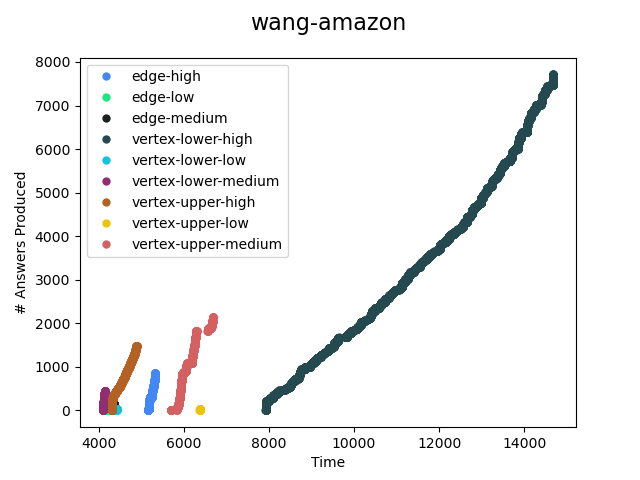
\includegraphics[width=1\linewidth, height=0.4\textheight]{experiments/diepfy/wang-amazon.png}
     \end{subfigure}
   \end{figure}
  \end{frame}

\begin{frame}[fragile]{E2: Average Excution Time}
  \begin{table}[H]
    \centering
    \resizebox{1\textwidth}{0.4\textheight}{%
    \begin{tabular}{|c|c|c|c|}
    \hline
     \textbf{Network} & \textbf{Scenario ID}  & \textbf{Average Execution Time} & \textbf{Standard deviation}\\
     \hline
     \multirow{6}{*}{Moreno Crime} & VL-L & $656$ ms & $13.0$ ms \\
     & VL-M & $669$ ms & $18.7$ ms \\ 
     & VL-H & $723$ ms & $72.2$ ms \\ 
     & E-L & $694$ ms & $4.7$ ms \\ 
     & E-M & $655$ ms & $14.9$ ms \\ 
     & E-H & $655$ ms & $21.1$ ms \\ 
     \hline
     \multirow{6}{*}{Opsahl UC Forum} & VL-L & $5.6$ s & $940$ ms \\
     & VL-M & $18.1$ s & $5.03$ s \\ 
     & VL-H & $70.8$ s & $2.03$ s \\ 
     & E-L & $41.9$ s & $2.87$ s \\ 
     & E-M & $26.7$ s & $5.63$ s \\ 
     & E-H & $26.2$ s & $4.05$ s \\
    \hline
    \multirow{6}{*}{Wang Amazon} & VL-L & $6.5$ s & $1.05$ s \\
    & VL-M & $5.91$ s & $994$ ms \\ 
    & VL-H & $10.2$ s & $2.66$ s \\ 
    & E-L & $6.4$ s & $1.08$ s \\ 
    & E-M & $5.71$ s & $863$ ms \\ 
    & E-H & $5.91$ s & $1.04$ s \\
   \hline
   \end{tabular}
    }
  \end{table}
  \end{frame}

  \iffalse
  \begin{frame}[fragile]{E2: Average Excution Time}
  \begin{figure}[H]
    \begin{center}
      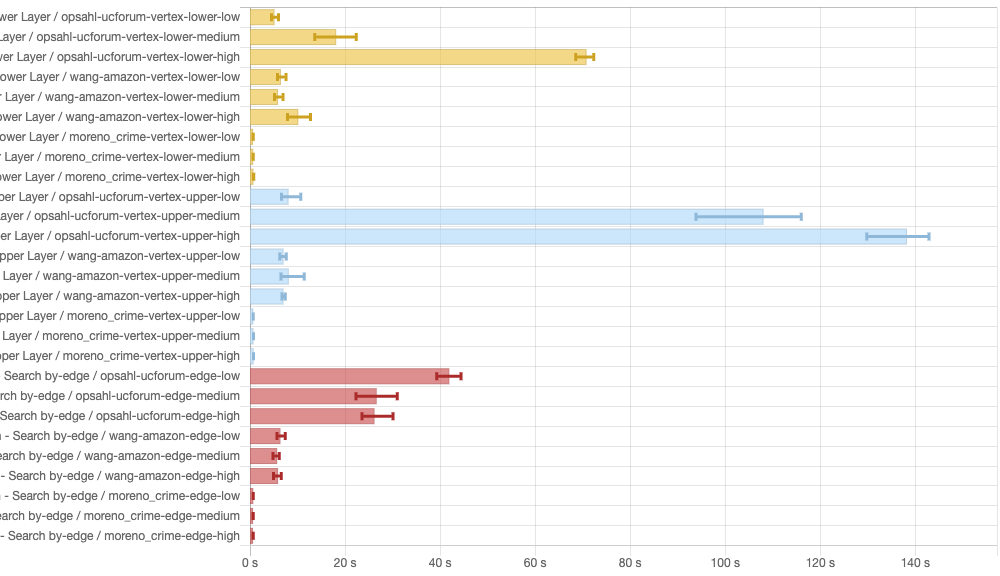
\includegraphics[width=1\textwidth]{experiments/bench_1}
    \end{center}
  \end{figure}
  \end{frame}
  \fi

\begin{frame}[fragile]{E2: Total Excution Time}
  \begin{figure}[H]
    \begin{center}
       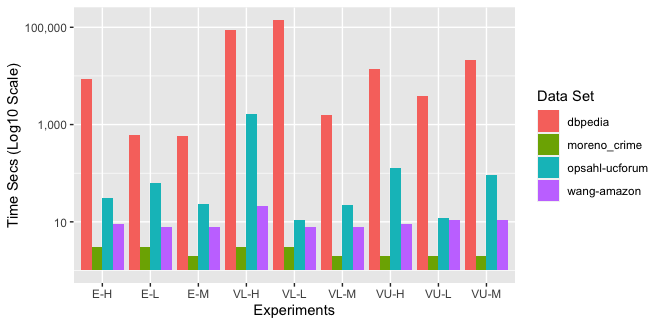
\includegraphics[width=1\textwidth] {experiments/execution_time_by_experiments}
    \end{center}
  \end{figure}
\end{frame}

\begin{frame}[fragile]{E3: Performance Analysis - Multithreading}
    \begin{figure}[!htp]
      \centering
      \begin{subfigure}[t]{0.45\textwidth}
        \begin{center}
          \textbf{General Overview}
        \end{center}
        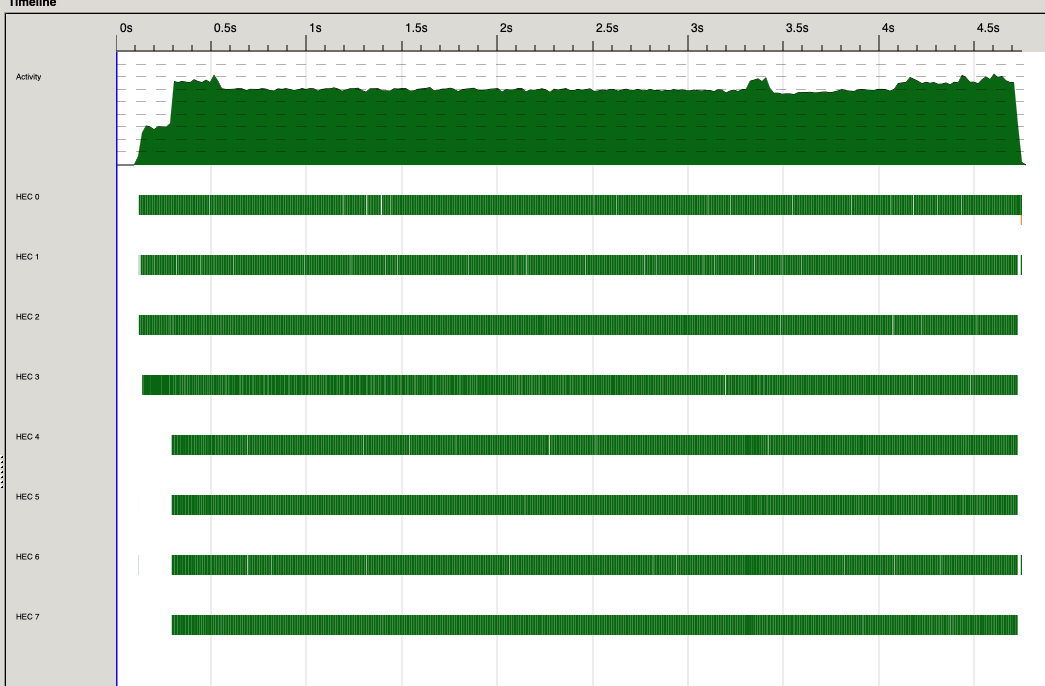
\includegraphics[width=1\linewidth, height=0.7\textheight]{experiments/thread/general_overview.png}
      \end{subfigure}\hfill
      \begin{subfigure}[t]{0.45\textwidth}
        \begin{center}
          \textbf{Middle Execution Time}
        \end{center}
        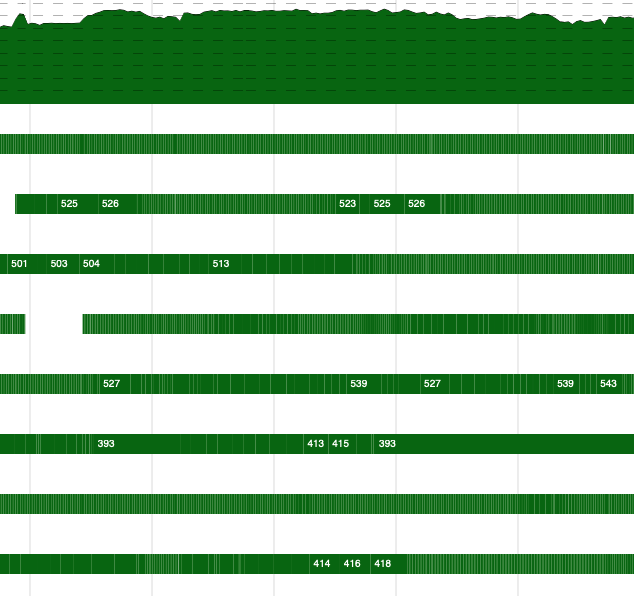
\includegraphics[width=1\linewidth, height=0.7\textheight]{experiments/thread/middle.png}
      \end{subfigure}
    \end{figure}
  \end{frame}


\begin{frame}[fragile]{E3: Performance Analysis - Memory Allocation}
  \begin{figure}[H]
    \begin{center}
      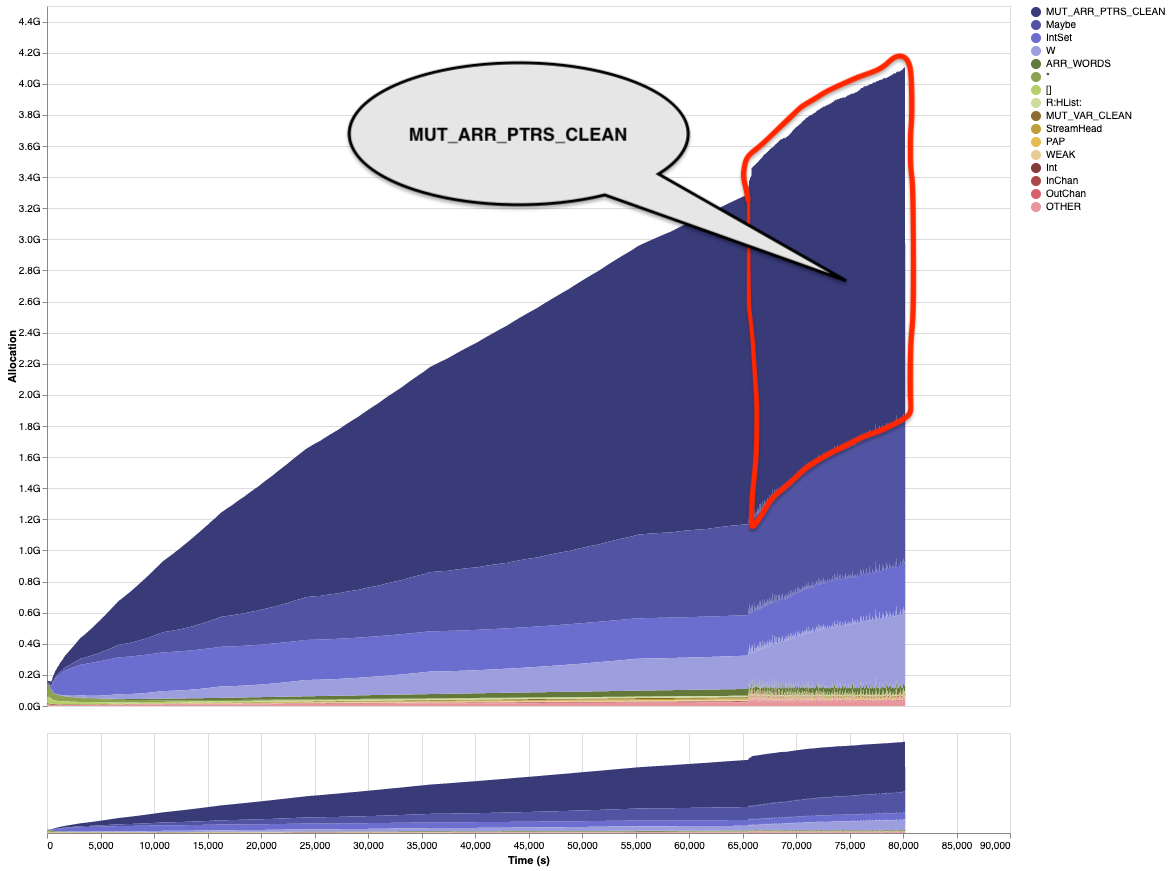
\includegraphics[width=0.8\textwidth] {experiments/mem/overview_1}
    \end{center}
  \end{figure}
\end{frame}

\begin{frame}[fragile]{Empirical Evaluation: Conclusions}
  \begin{itemize}
    \setlength\itemsep{1.5em}
    \item Results of \textbf{dief$@$t} and \textbf{dief$@$k} metrics indicates continuous behavior.
    \item \textbf{High values} of \textbf{\emph{Average Running Time}} and \textbf{\emph{Total Running Time}} are suggesting an effective implementation of a \emph{pay-as-you-go} model of \acrshort{dpbt}.
    \item Results in \texttt{ThreadScope} tool indicates an \textbf{efficient use of the parallel model}.
    \item Results in \texttt{eventlog2html} tool indicates \textbf{efficient memory consumption}.
  \end{itemize} 
\end{frame}
